\documentclass{report}
\usepackage[spanish]{babel}
\usepackage{graphicx}
\usepackage{mathtools}


\begin{document}

\tableofcontents

\chapter{Incertidumbre}

Hay dos caminos, el metodo MONTECARLO que es utilizando una aproximacion discreta.
$$\sigma = \sqrt{\sum_{i=1}^{N} \frac{A_{p_i}^2}{N-1} }$$


Camino dos: hallar la relacion entre $\sigma$ y la desv estandar de exactitud y resolucion.

$$\sigma^2 = \sigma_{exactitud}^2 + \sigma_{resolucion}^2 $$
Podemos hallar la desviacion estandar de la exactitud y la resolucion usando una formula que viene de estadistica/probabilidad

$$\sigma_x^2 = \int_{-\infty}^{+\infty}{(x-\mu)^2f(x)dx}$$
$$\sigma_{exactitud} = \frac{exactitud}{\sqrt{3}}$$
$$\sigma_{resolucion} = \frac{resolucion}{2\sqrt{3}}$$


\section{Calculo de incertidumbre (Metodo GUM - clasico)}


$$y = f(x_1,x_2,...,x_n)$$
Ejemplo: $R = \frac{V}{I} \Rightarrow R = f(V,I)$

\subsection{Incertidumbre tipo A ("Estadistica")}

Hago siempre lo mismo e igual varia.
Se toman $M$ medidas $\Rightarrow y_1,...,y_M$

$$U_A = \frac{\sigma_A}{\sqrt{M}}$$
$$\sigma_A = \sqrt{\sum_{i=1}^M{\frac{(y_i - \bar{y})^2}{M-1}}}$$
$$\bar{y} = \frac{\sum_{i=1}^M{y_i}}{M}$$


\subsection{Incertidumbre tipo B ("No estadistico")}

Apartamientos por el sistema de medida.

$$y = \underbrace{y_0}_{f(p_0)} + \frac{\partial{f}}{\partial x_1}
	\rvert_{p=p_0} (x_1 - x_0) + ... + \frac{\partial{f}}{\partial x_n}
	\rvert_{p=p_0} (x_N - x_{n_0})$$

Aca $p_0$ es el promedio de los valores medidos


Truncamos el Taylor en orden 2, ademas:
$$C_i = \frac{\partial{f}}{\partial{x_i}}$$

$$\Delta y =C_1\Delta x_1 + ... + C_n \Delta x_n$$

$$u(x_k) = ~\text{propagacion de varianzas en todas las fuentes}$$
Para esto miramos la exactitud y resolucion de cada variable
$$\boxed{U_{B} = \sqrt{\sum_{k=1}^{N}{C_K^2}\cdot {u(x_k)}^2}}$$


\subsection{Incertidumbre combinada}

$$U_C = \sqrt{U_A^2 + U_B^2}$$

\subsection{Incertidumbre expandida}

$$U_E = K \cdot U_C$$
$K$ es el factor de cobertura.
Usualmente $K = 2$ (95% de confianza $\to$ distribucion normal)

Resultado de la medida: $\bar{y} \pm U_E$

\section{Metedo Montecarlo}

Para el metodo de Montecarlo hacemos lo siguiente:
\begin{itemize}
	\item Generamos distribucion normal de valores de $m$
	\item Generamos distribucion normal de valores de $V$
	\item Luego intentamos hallar distribucion (normal) de valores de $\delta$ donde $$\delta_j = \frac{m_j}{V_j}$$
\end{itemize}

Si tenemos una variable $X$ que aparenta ser normal, esto es: $X\sim N(\mu ,\sigma^2)$ \
Entonces podemos hacer un cambio de variable $Z=\frac{X-\mu}{\sigma}$ \
$$\Rightarrow Z \sim N(0,1)$$
$$X = Z\sigma + \mu$$



\chapter{Osciloscopio}





\chapter{Voltimetro}

\section{Instrumentos analógicos}
Siguen vigentes porque son baratos y muy sensibles entonces se pueden construir instrumentos que miden con muy buena precision de forma barata.
Tambien son demandados por las insdustrias.

\subsection{Funcionanmiento}
Tenemos un iman permanente con una bobina movil. A traves de la bobina movil circula la corriente, lo que induce una fuerza por ley de Faraday y esto genera un par magnético que rota la aguja. \\
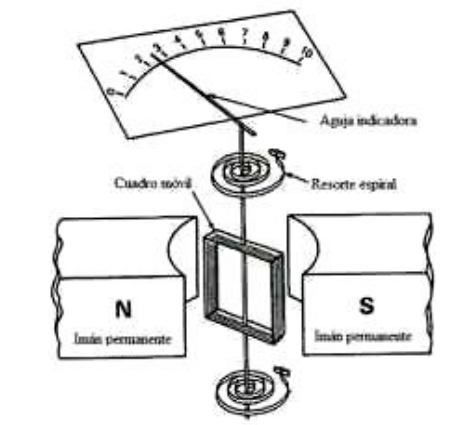
\includegraphics[width=8cm]{../Assets/voltimetro.png} \\
Cuando la bobina gira, arrastra la espira en cortocircuito que, por moverse en un campo magnético tendrá una f.e.m inducida y por tratarse de un circuito cerrado circula una intensidad inducida, que reacciona con el campo magnético generando un par que se opone al movimiento y que se llama AMORTIGUAMIENTO.

\subsection{Ecuacion diferencial de su movimiento}
\[
	J \frac{\partial^2{\theta}}{\partial{t^2}} = Gi - D \frac{\partial{\theta}}{\partial{t}} - k_r\theta
\]
Donde $J$ es el momento de inercia del rotor.

\section{Ley de respuesta de respuesta}
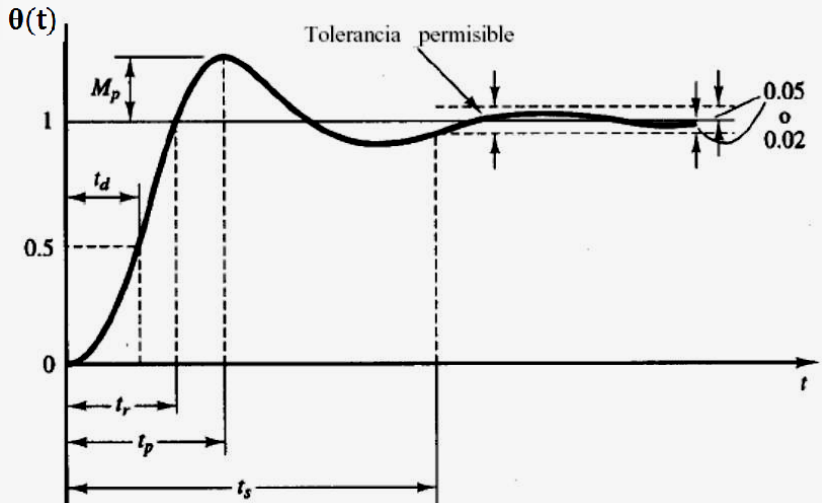
\includegraphics[width=8cm]{../Assets/instrumentos_analogicos_ley_de_respuesta.png}



\end{document}
